\documentclass{article}
\usepackage{tikz}
\usepackage{physics}
\usetikzlibrary{decorations.pathmorphing}
\usetikzlibrary{decorations.markings}
\usetikzlibrary{arrows.meta}

\begin{document}

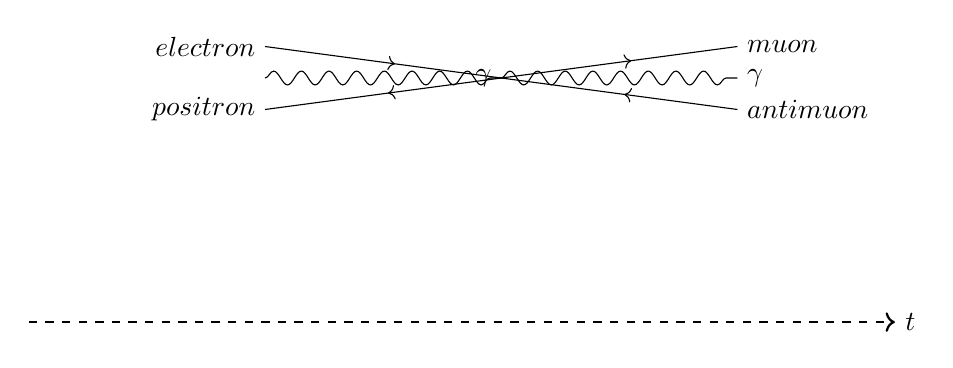
\begin{tikzpicture}[
  fermion/.style={draw=black, postaction={decorate}, decoration={markings,mark=at position .55 with {\arrow[black]{>}}}},
  antifermion/.style={draw=black, postaction={decorate}, decoration={markings,mark=at position .55 with {\arrow[black]{<}}}},
  photon/.style={decorate, decoration={snake}, draw=black},
  gluon/.style={decorate, decoration={coil, amplitude=4pt, segment length=5pt}, draw=black},
  weak/.style={decorate, decoration={snake, amplitude=1pt}, draw=black},
  time axis/.style={->, thick, draw=black, dashed}
]

% Time axis
\draw[time axis] (-1,-2) -- (10,-2) node[right] {$t$};

%% SPECTATOR PARTICLES
% Spectator particles (straight horizontal lines at the top)


% Position counter for interactions (starts below spectators)


%% FLAVOR CHANGING INTERACTIONS


%% STRONG INTERACTIONS


%% EM INTERACTIONS

  
  
  % Initial EM pairs
  
    \coordinate (em_i11) at (2,1.5);
    \coordinate (em_i21) at (2,0.7);
    \coordinate (em_mid1) at (5,1.1);
    
    \draw[fermion] (em_i11) -- (em_mid1);
    \draw[antifermion] (em_i21) -- (em_mid1);
    \draw[photon] (em_mid1) -- (8,1.1) node[right] {$\gamma$};
    
    \node[left] at (em_i11) {$electron$};
    \node[left] at (em_i21) {$positron$};
    
    
  
  
  % Final EM pairs
  
    \coordinate (em_f1) at (5,1.1);
    \coordinate (em_o11) at (8,1.5);
    \coordinate (em_o21) at (8,0.7);
    
    \draw[photon] (2,1.1) -- (em_f1) node[left] {$\gamma$};
    \draw[fermion] (em_f1) -- (em_o11);
    \draw[antifermion] (em_f1) -- (em_o21);
    
    \node[right] at (em_o11) {$muon$};
    \node[right] at (em_o21) {$antimuon$};
    
    
  


%% WEAK INTERACTIONS


\end{tikzpicture}

\end{document}